\section{Vježba 3: Houghova transformacija}

\subsection{Opis vježbe}
Potrebno je pomoću, prethodno kalibrirane, web kamere uslikati objekt
kvadratnog oblika koji je postavljen na milimetarskom papiru na stolu.
Primjenom Houghove transformacije (HT) treba odrediti parametre \(\rho
\) i \( \theta \)najdominantnijeg pravca, koji odgovara jednom od rubova objekta
na slici. Pod najdominantnijim pravcem podrazumijeva se pravac kojem
pripada najveći broj 'glasova' u akumulacijskoj ravnini. Implementacija
HT u biblioteci OpenCV vraća popis detektiranih pravaca koji su
razvrstani prema broju 'glasova' počevši od najdominantnijeg. Primjenom
odgovarajuće transformacije, odrediti \(\rho i \theta \)tog pravca u
koordinatnom sustavu milimetarskog papira. Provjeriti koliko je
odstupanje dobivenog pravca od stvarnog (odgovarajućeg) ruba objekta.

\subsection{Kalibracija kamere}
Cijenovna prihvatljivosti web kamera ima
svoju negativnu stranu, a to je značajna distorzija. 
Postoji radijalna (\textit{fisheye} efekt i tangencijalna (leće kamere
nisu u savršeno paralelene s ravninom slikanja) distorzija. Zato
kalibracijom kamere možemo rješiti te nedostatke. Isto tako kalibracijom
možemo odrediti vezu između piksela i milimetara.

Za kalibraciju smo koristili program koji se kompajlira prilikom
kompajliranja OpenCV biblioteke. Pomoću njega smo dobili koeficiente
distorzije i matricu kamere. Ti podatke program dobije računanjem
jednostavnih geometrijskih jednađbi nad primjerom crno bijele šahovske ploče.

\begin{figure}[h]
\centering
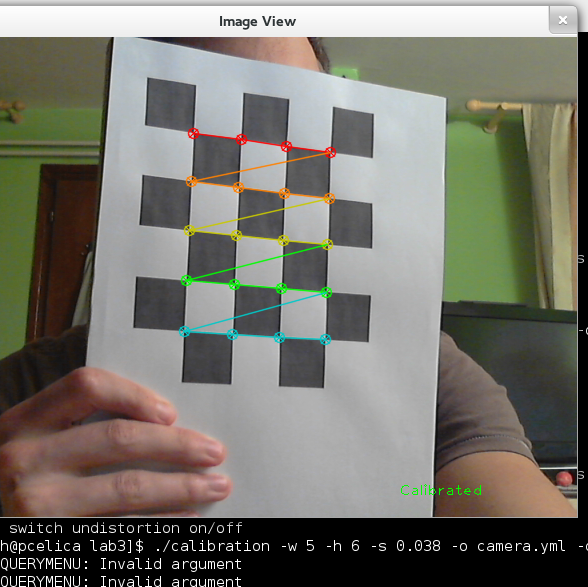
\includegraphics[scale=0.4]{images/lab3-01-calib.png}
\caption{Kalibracija kamere}
\label{fig:lab3-01-calib}
\end{figure}

\newpage
\subsection{Objašnjenje programa}

\subsubsection{Kontrola programa}

Prilikom pokretanja programa iz komandne linije potrebno je 
predati programu putanju do slike (argv[1]) u protivnom se program 
nece pokrenuti. \\
\begin{lstlisting}[language=C,caption={Kontrola programa tipkovnicom}]
while (1){
    char c = waitKey(10);
    switch(c) {
            case 'c':
                initCamera( );
                break;
            case 'o':
                camera = false;
                break;
            case 's':
                cam_frame.copyTo( ss_img );
                namedWindow( "snapshot", CV_WINDOW_AUTOSIZE );
                imshow( "snapshot", ss_img );
                cout << " Setting MouseCallback getPoints " << endl;
                setMouseCallback( "snapshot", getPoints, 0 );
                break;
            case 'h':
                cannyEdge( ss_img, ss_box );
                break;
            case 'H':
                if(!canny_out.data){
                    cout << "pozivi canny" << endl;
                    break;
                }
                callHoughTransform( );
                break;
\end{lstlisting}

\begin{itemize}
    \item Pokrenut kameru pritiskom na ``c''
    \item Uslikati objekt na milimetarskom papiru s ``s''
    \item Označiti (klikom) četiri ugla milimetarskog papira
    \item Ugasiti kameru pritsikom na ``o''
    \item Pokrenuti filtiranje slike pritiskom na ``h''
    \item Pozvati houghovu transformaciju pritiskom na ``H''
\end{itemize}


\subsubsection{Houghova transformacija}
Houghovu transformaciju, odnosno detektiranje linija je implementirano u
funkciji \textit{cv::HoughLines()}. Njoj smo predali sliku uslikanu
kamerom i detektiranom linijom. Funkcija nam tada vraća parametre 
\(\rho \) i \( \theta \) u 2D slici iz kojih određujemo parametre 
\(\rho \)' i \( \theta\)' u 3D prostoru.

\begin{figure}[h]
\centering
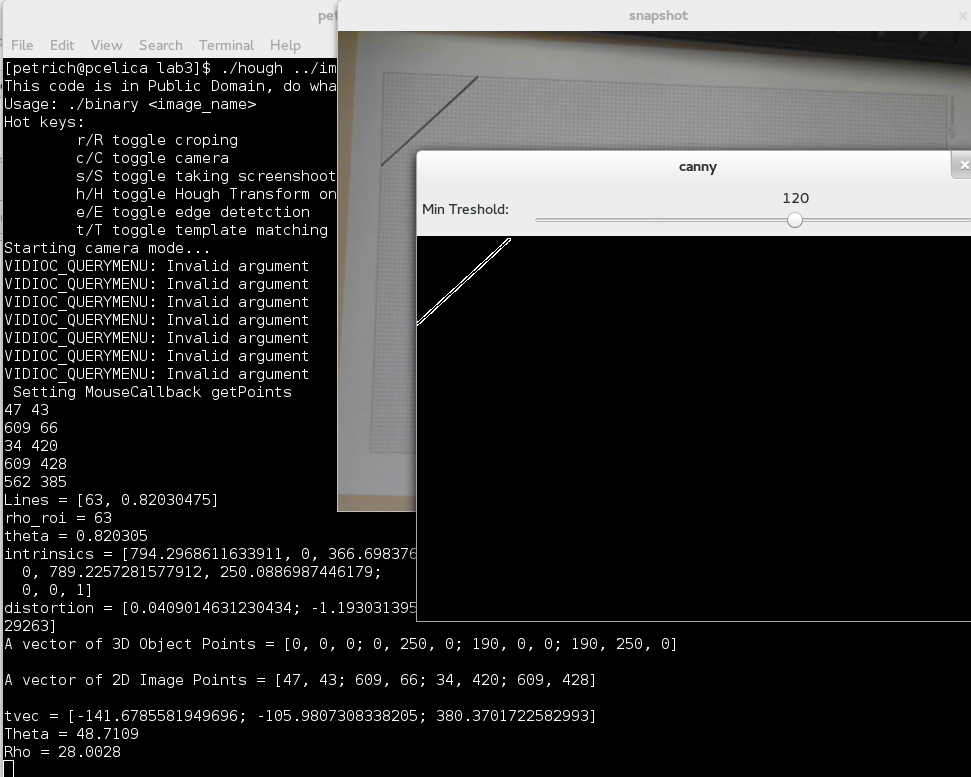
\includegraphics[scale=0.4]{images/lab3-02-ht.png}
\caption{Houghova transformacija}
\label{fig:lab3-02-ht}
\end{figure}

\begin{lstlisting}[language=C,caption={Racunanje parametra ro i theta}]
void callHoughTransform( ){
    vector<Vec2f> lines;
    HoughLines( canny_out, lines, 1, CV_PI/180, 100, 0, 0 );
    cout << "Lines = " << Mat( lines ) << endl;
    float rho, rho_roi, theta;
    rho_roi= lines[0][0];
    theta = lines[0][1];
    // prebacivanje u k.s. slike
    rho = rho_roi + pt1.x * cos( theta ) + pt1.y * sin( theta );
    cout << "rho_roi = " << rho_roi << endl;
    cout << "theta = " << theta << endl;
    // ucitavanje parametara kamere
    FileStorage fs("calib/cam.xml", FileStorage::READ);
    Mat intrinsics(3, 3, CV_32F ); 
    Mat distortion( 5, 1, CV_32F );
    fs["camera_matrix"] >> intrinsics; //3*3
    fs["distortion_coefficients"] >> distortion; //4*1, kod mene 5*1
    cout << "intrinsics = " << intrinsics <<  endl;
    cout << "distortion = " << distortion <<  endl;
    vector<Point3f> objectPoints(4);
    objectPoints[0] = Point3f( 0, 0, 0 );
    objectPoints[1] = Point3f( 0, 250, 0 );
    objectPoints[2] = Point3f( 190, 0, 0 );
    objectPoints[3] = Point3f( 190, 250, 0 );
    cout << "A vector of 3D Object Points = " << objectPoints << endl << endl;
    cout << "A vector of 2D Image Points = " << imagePoints << endl << endl;
    Mat rvec( 1, 3, CV_32F );
    Mat tvec( 1, 3, CV_32F );
    Mat R( 3, 3, CV_32F );
    Mat A( 3, 3, CV_32F );
    Mat B( 3, 1, CV_32F );
    solvePnP( Mat(objectPoints), Mat(imagePoints), intrinsics, distortion, rvec, tvec, false );
    cout << "tvec = " << tvec <<  endl;
    Rodrigues( rvec, R );
    A = intrinsics * R; // A = P * R
    B = intrinsics * tvec; // B = P * t
    double lambdaX, lambdaY, lambdaRo, rho_crtano, theta_crtano;
    // lambdaX = a11*cos(theta) + a21*sin(theta) - ro*a31
    lambdaX = A.at<double>(0,0) * cos(theta) + A.at<double>(1,0) * sin(theta) - rho * (A.at<double>(2,0));
    // lambdaY = a12*cos(theta) + a22*sin(theta) - ro*a32
    lambdaY = A.at<double>(0,1) * cos(theta) + A.at<double>(1,1) * sin(theta) - rho * (A.at<double>(2,1));
    // lamdbaRo = b3*ro - b1*cos(theta) - b2*sin(theta) 
    lambdaRo = rho * (B.at<double>(2)) - B.at<double>(0) * cos(theta) - B.at<double>(1) * sin(theta); 
    theta_crtano = atan2( lambdaY, lambdaX );
    rho_crtano = lambdaRo / sqrt( lambdaX * lambdaX + lambdaY * lambdaY );
    cout << "Theta = " << theta_crtano*180/CV_PI << endl;
    cout << "Rho = " << rho_crtano << endl;
}

\end{lstlisting}

\subsection{Zaključak}


